\documentclass[12pt, oneside]{article}

\usepackage[letterpaper, scale=0.8, centering]{geometry}
\usepackage{fancyhdr}
\setlength{\parindent}{0em}
\setlength{\parskip}{1em}

\pagestyle{fancy}
\fancyhf{}
\renewcommand{\headrulewidth}{0pt}
\rfoot{{\footnotesize Copyright Daniel Grier / Mia Minnes, 2023, Version \today~(\thepage)}}

\usepackage{titlesec}

\author{CSE105Sp23}

\newcommand{\instructions}{{\bf For all HW assignments:} Weekly homework 
may be done individually or in groups of up to 3 students. 
You may switch HW partners for different HW assignments. 
The lowest HW score will not be included in your overall HW average. 
Please ensure your name(s) and PID(s) are clearly visible on the first page of your homework submission 
and then upload the PDF to Gradescope. If working in a group, submit only one submission per group: 
one partner uploads the submission through their Gradescope account and then adds the other group member(s) 
to the Gradescope submission by selecting their name(s) in the ``Add Group Members" dialog box. 
You will need to re-add your group member(s) every time you resubmit a new version of your assignment.
 Each homework question will be graded either for correctness (including clear and precise explanations and 
 justifications of all answers) or fair effort completeness. You may only collaborate on HW with CSE 105 students 
 in your group; if your group has questions about a HW problem, you may ask in drop-in help hours or post a private 
 post (visible only to the Instructors) on Piazza.

All submitted homework for this class must be typed. 
You can use a word processing editor if you like (Microsoft Word, Open Office, Notepad, Vim, Google Docs, etc.) 
but you might find it useful to take this opportunity to learn LaTeX. 
LaTeX is a markup language used widely in computer science and mathematics. 
The homework assignments are typed using LaTeX and you can use the source files 
as templates for typesetting your solutions.
To generate state diagrams of machines, we recommend using Flap.js
or JFLAP. Photographs of clearly hand-drawn diagrams may also be used. We recommend that you
submit early drafts to Gradescope so that in case of any technical difficulties, at least some of your
work is present. You may update your submission as many times as you'd like up to the deadline.


{\bf Integrity reminders}
\begin{itemize}
\item Problems should be solved together, not divided up between the partners. The homework is
designed to give you practice with the main concepts and techniques of the course, 
while getting to know and learn from your classmates.
\item You may not collaborate on homework with anyone other than your group members.
You may ask questions about the homework in office hours (of the instructor, TAs, and/or tutors) and 
on Piazza (as private notes viewable only to the Instructors).  
You \emph{cannot} use any online resources about the course content other than the class material 
from this quarter -- this is primarily to ensure that we all use consistent notation and
definitions (aligned with the textbook) and also to protect the learning experience you will have when
the `aha' moments of solving the problem authentically happen.
\item Do not share written solutions or partial solutions for homework with 
other students in the class who are not in your group. Doing so would dilute their learning 
experience and detract from their success in the class.
\end{itemize}

}

\newcommand{\gradeCorrect}{({\it Graded for correctness}) }
\newcommand{\gradeCorrectFirst}{\gradeCorrect\footnote{This means your solution 
will be evaluated not only on the correctness of your answers, but on your ability
to present your ideas clearly and logically. You should explain how you 
arrived at your conclusions, using
mathematically sound reasoning. Whether you use formal proof techniques or 
write a more informal argument
for why something is true, your answers should always be well-supported. 
Your goal should be to convince the
reader that your results and methods are sound.} }
\newcommand{\gradeComplete}{({\it Graded for completeness}) }
\newcommand{\gradeCompleteFirst}{\gradeComplete\footnote{This means you will 
get full credit so long as your submission demonstrates honest effort to 
answer the question. You will not be penalized for incorrect answers. 
To demonstrate your honest effort in answering the question, we ask 
that you include your attempt to answer *each* part of the question. 
If you get stuck with your attempt, you can still demonstrate 
your effort by explaining where you got stuck and what 
you did to try to get unstuck.} }

\usepackage{tikz}
\usetikzlibrary{automata,positioning,arrows}

\usepackage{amssymb,amsmath,pifont,amsfonts,comment,enumerate,enumitem}
\usepackage{currfile,xstring,hyperref,tabularx,graphicx,wasysym}
\usepackage[labelformat=empty]{caption}
\usepackage[dvipsnames,table]{xcolor}
\usepackage{multicol,multirow,array,listings,tabularx,lastpage,textcomp,booktabs}

% NOTE(joe): This environment is credit @pnpo (https://tex.stackexchange.com/a/218450)
\lstnewenvironment{algorithm}[1][] %defines the algorithm listing environment
{   
    \lstset{ %this is the stype
        mathescape=true,
        frame=tB,
        numbers=left, 
        numberstyle=\tiny,
        basicstyle=\rmfamily\scriptsize, 
        keywordstyle=\color{black}\bfseries,
        keywords={,procedure, div, for, to, input, output, return, datatype, function, in, if, else, foreach, while, begin, end, }
        numbers=left,
        xleftmargin=.04\textwidth,
        #1
    }
}
{}
\lstnewenvironment{java}[1][]
{   
    \lstset{
        language=java,
        mathescape=true,
        frame=tB,
        numbers=left, 
        numberstyle=\tiny,
        basicstyle=\ttfamily\scriptsize, 
        keywordstyle=\color{black}\bfseries,
        keywords={, int, double, for, return, if, else, while, }
        numbers=left,
        xleftmargin=.04\textwidth,
        #1
    }
}
{}

\newcommand\abs[1]{\lvert~#1~\rvert}
\newcommand{\st}{\mid}

\newcommand{\A}[0]{\texttt{A}}
\newcommand{\C}[0]{\texttt{C}}
\newcommand{\G}[0]{\texttt{G}}
\newcommand{\U}[0]{\texttt{U}}

\newcommand{\cmark}{\ding{51}}
\newcommand{\xmark}{\ding{55}}


\newcommand{\SUBSTRING}{\textsc{Substring}}
\newcommand{\REP}{\textsc{Rep}}
\newcommand{\blank}{\scalebox{1.5}{\textvisiblespace}}


\title{HW2 : Regular Languages and Automata Constructions}
\date{Due: April 18th at 5pm (no penalty late submission until 8am next morning), via Gradescope}

\begin{document}
\maketitle
\thispagestyle{fancy}

You will practice designing multiple representations of regular languages and working with general 
constructions of automata to demonstrate the richness of the class of regular languages.

\textit{Resources}: To review the topics you are working with for this assignment, see the 
class material from Week 1 and Week 2. We will post frequently asked questions and our answers to them in a pinned Piazza post.

\textit{Reading and extra practice problems}: Sipser Section 1.1, 1.2, 1.3. 
Chapter 1 exercises 1.4, 1.5, 1.6, 1.7, 1.8, 1.9, 1.10, 1.11, 1.12, 1.14, 1.15, 1.16, 1.17, 1.19, 1.20, 1.21, 1.22.

\textit{Key Concepts:} Regular expressions, language described by a regular expression, 
deterministic finite automata (DFAs), regular languages, closure of the class of regular languages under certain operations, 
nondeterministic finite automata (NFA).

\instructions

You will submit this assignment via Gradescope
(\href{https://www.gradescope.com}{https://www.gradescope.com}) 
in the assignment called ``hw2CSE105Sp23''.

\textbf{Assigned questions}

\begin{enumerate} 

%%%%%%%%%%% PROBLEM 1 %%%%%%%%%%%

\item \textbf{It can be hard to give a good complement} (15 points): \\
For any language $L \subseteq \Sigma^*$, recall that we define its \emph{complement} as 
$$\overline{L} := \Sigma^* - L = \{w \in \Sigma^* \mid w \notin L\}$$ That is, the complement of $L$ 
contains all and only those strings which are not in $L$. Our notation for regular expressions does not 
include the complement symbol. However, 
it turns out that the complement of a language described by a regular expression is guaranteed to also be describable by a 
(different) regular expression. For example, over the alphabet $\Sigma = \{0,1\}$, the complement of the language described 
by the regular expression $\Sigma^* 0$ is described by the regular expression $\varepsilon \cup \Sigma^*1$
because any string that does not end in $0$
must either be the empty string or end in $1$.

For each of the regular expressions $R$ over the alphabet $\Sigma = \{0,1\}$ below, write the regular 
expression for~$\overline{L(R)}$. Your regular expressions may use the symbols
$\varnothing$, $\varepsilon$, $0$, $1$, and the 
following operations to combine them: union, concatenation, 
and Kleene star.

Briefly justify why your solution for each part works by giving plain English descriptions of the language 
described by the regular expression and of its complement and connecting them to the regular 
expression via relevant definitions. An English description that is more 
detailed than simply negating the description in the original language will likely be helpful in the justification.

\begin{enumerate}
    \item\gradeCorrectFirst $(\Sigma \Sigma)^*$
    \item\gradeCorrect $\Sigma^* 11 \Sigma^*$
    \item\gradeCorrect $0^* 1 0^* 1 0^*$
\end{enumerate}

%%%%%%%%%%% PROBLEM 2 %%%%%%%%%%%

\item \textbf{Closure of the class of regular languages under intersection} (12 points): \\
For this question, let $\Sigma = \{0,1\}$.
Recall the DFA over $\Sigma$ from the previous homework:
\begin{center}
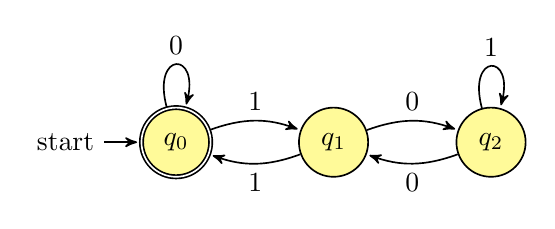
\begin{tikzpicture}[->,>=stealth',shorten >=1pt, auto, node distance=2cm, semithick]
  \tikzstyle{every state}=[text=black, fill=yellow!40]

  \node[initial,state, accepting] (q0)                    {$q_0$};
  \node[state]         (q1) [right of=q0] {$q_1$};
  \node[state]         (q2) [right of=q1] {$q_2$};

  \path (q0) edge  [loop above] node {$0$} (q0)
  		edge [bend left=20] node {$1$} (q1)
	(q1) edge [bend left=20] node {$0$} (q2)
		edge [bend left=20] node {$1$} (q0)
	(q2) edge [loop above] node {$1$} (q2)
		edge [bend left=20] node {$0$} (q1)
 ;
\end{tikzpicture}
\end{center}
We'll call the language recognized by the DFA above $A$.
Let's also define a new language $B \subseteq \Sigma^*$ to be 
the language recognized by the DFA 
over $\Sigma$ with state diagram below:
\begin{center}
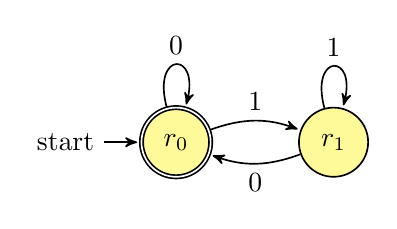
\begin{tikzpicture}[->,>=stealth',shorten >=1pt, auto, node distance=2cm, semithick]
  \tikzstyle{every state}=[text=black, fill=yellow!40]

  \node[initial,state, accepting] (q0)                    {$r_0$};
  \node[state]         (q1) [right of=q0] {$r_1$};

  \path (q0) edge  [loop above] node {$0$} (q0)
  		edge [bend left=20] node {$1$} (q1)
	(q1) edge [loop above] node {$1$} (q1)
		edge [bend left=20] node {$0$} (q0)
 ;
\end{tikzpicture}
\end{center}

\begin{enumerate}
    \item\gradeCorrect Using the construction for the intersection of two regular languages (Sipser page 46), 
    draw the state diagram for a DFA recognizing the intersection of the languages $A$ and $B$. The labels of 
    each one of your states should be the ordered pair of labels for the states from the two machines above. 
    Your diagram should have $6$ states.
    \item\gradeComplete In this part of the problem, you will prove that the general construction for the DFA 
    recognizing intersection of two languages that 
    you used in part (a) does not always produce a DFA
    with the smallest number of states possible. 
    You will do this by giving one counterexample (that combined with your work in part (a), 
    proves the general claim). Your task: design a DFA with exactly 4 states that recognizes 
    the language $A \cap B$. Briefly justify why your design works by describing the role of each state
    of your DFA and relating it to a plain English description of the language resulting from the intersection.
    \item\gradeCorrect  Later in the class we will learn that there are some languages which are not regular, 
    and in fact, we will learn specific techniques to prove that certain languages are not regular. 
    For the moment, however, we can already investigate closure properties of the class of regular 
    languages just by knowing that a non-regular language exists. 

    We know (from the textbook and our work in class) that if $L$ and $K$ are regular languages, 
    then $L \cap K$ is regular (for arbitrary languages $L$ and $K$). Prove that the converse of this statement is false; that is, 
    give a counterexample by giving a specific regular language $L$ so that
    for each non-regular language $X$, $L \cap X$ is regular (even though $X$ isn't).

    In your solution, justify why $L$ is regular 
    and why $L \cap X$ is regular (for arbitrary $X$) using relevant definitions.
\end{enumerate}


{\it (Challenge question, not graded) Prove/disprove: For 
any language $L$ over $\Sigma^*$, $L \cap B$ is regular implies $L$ is regular, where $B$ is the specific language from part (a) 
and (b) of Problem 2.}

%%%%%%%%%%% PROBLEM 3 %%%%%%%%%%%
\item {\bf Closure of the class of regular languages under} \SUBSTRING~(16 points): \\
Let $\Gamma = \{0,1,2\}$. From the previous homework, recall the function $\SUBSTRING$ that 
has domain and codomain
$\mathcal{P}(\Gamma^*)$, 
where, for each language $K$ over $\Gamma$,
$$\SUBSTRING(K) := \{ w \in \Gamma^* \mid \text{there exist } a,b \in \Gamma^* \text{ such that } awb \in K\}$$
\begin{enumerate}
\item \gradeCorrect Consider the NFA over $\Gamma$ with state diagram:
\begin{center}
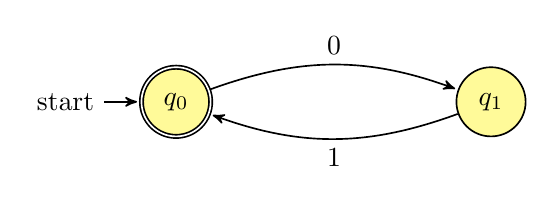
\begin{tikzpicture}[->,>=stealth',shorten >=1pt, auto, node distance=2cm, semithick]
  \tikzstyle{every state}=[text=black, fill=yellow!40]

  \node[initial,state, accepting] (q0)                    {$q_0$};
  \node		     (c)   [right of=q0] {};
  \node[state]         (q1) [right of=c] {$q_1$};
  
  \path (q0) edge [bend left=20] node {$0$} (q1)
	(q1) 	edge [bend left=20] node {$1$} (q0)
 ;
\end{tikzpicture}
\end{center}
We'll call the language recognized by the NFA above $C$.
Fill in the blanks below: 
\begin{itemize}
    \item An example of a string over $\Gamma$ that is in $C$
    {\bf and} is in $\SUBSTRING(C)$ is \underline{\phantom{\hspace{1in}}} because 
    \underline{\phantom{\hspace{1in}}}
    \item An example of a string over $\Gamma$ that is in $C$
    {\bf and} is {\bf not} in $\SUBSTRING(C)$ is \underline{\phantom{\hspace{1in}}} because 
    \underline{\phantom{\hspace{1in}}}
    \item An example of a string over $\Gamma$ that is {\bf not} in $C$
    {\bf and} is in $\SUBSTRING(C)$ is \underline{\phantom{\hspace{1in}}} because 
    \underline{\phantom{\hspace{1in}}}
    \item An example of a string over $\Gamma$ that is {\bf not} in $C$
    {\bf and} is {\bf not} in $\SUBSTRING(C)$ is \underline{\phantom{\hspace{1in}}} because 
    \underline{\phantom{\hspace{1in}}}
\end{itemize}
For each item, you'll either fill in a specific string 
and a justification that refers back to the relevant 
definitions, or you'll write ``impossible'' for the first 
part of the sentence and justify why it's impossible to find such 
an example referring back to the relevant definitions.
\item\gradeComplete Prove 
that the class of regular languages is closed under the $\SUBSTRING$ operation. Namely, give a general construction 
that takes an arbitrary NFA and constructs
 an NFA that recognizes the result of applying $\SUBSTRING$
 to the language recognized by the original machine. 
You can describe your construction in words and/or
draw a picture to illustrate your construction.
You do not have to write down a formal specification.

\item\gradeComplete Draw the state diagram of an 
NFA over $\Gamma$ that recognizes $\SUBSTRING(C)$ (for 
$C$ the language from part (a) of this Problem), using
your construction from part (b) of this Problem, or manually
constructing it. 
Describe the computation(s) of this NFA for each of the 
sample strings you gave in part (a).
\end{enumerate}

%%%%%%%%%%% PROBLEM 4 %%%%%%%%%%%
\item {\bf Closure of the class of regular star-free languages under} \REP~(7 points):\\
A language is said to be \emph{star-free} whenever it can be described by a regular expression that 
has no Kleene star operations, but where complement operation can be 
incorporated into the expression as many times as you like. 
For example, the language $$\{\varepsilon, 0010\}$$ is star-free because it can be described
by $\varepsilon \cup 0010$ which does not use the Kleene star operation symbol.
\begin{enumerate}
    \item\gradeCorrect Prove that the set of all strings 
    over $\Gamma = \{0,1,2\}$ is star-free. A complete solution
    will give an expression that describes this language 
    that does not use Kleene star but may incoporate the complement
    expression as many times as you like, along 
    with a justification that refers back to relevant definitions.
    \item\gradeComplete Prove that every finite language is star-free.
    \item\gradeComplete Let $\Sigma = \{0,1\}$. From the previous
    homework, recall the function $\REP$ that has domain 
    $\mathcal{P}(\Sigma^*)$ and codomain $\mathcal{P}(\Gamma^*)$, 
    where, for each language $L$ over $\Sigma$,
    \begin{align*}
        \REP(L) &:= \{ w \in \Gamma^* \mid \text{between every 
    pair of successive $2$'s in $w$ is a string in $L$}\}
    \end{align*}
    
    Show that $\REP(L)$ is a regular and star-free language 
    whenever $L$ is a regular and star-free language. That is, 
    given an expression $R$ describing $L$, write a regular 
    expression for $\REP(L)$ using only the regular expressions 
    $R$, $\varnothing$, $\varepsilon$, $0$, $1$, $2$, and the 
    following operations to combine them: union, concatenation, 
    and complement. You may assume that $\overline{R}$
    describes $\Sigma^* -L(R)$, that is, the complement for the regular expression $R$ over the alphabet $\Sigma$ is itself 
    a language over $\Sigma$. 
\end{enumerate}

%%%%%%%%%%% END PROBLEMS  %%%%%%%%%%%
\end{enumerate}

\end{document}